\documentclass[a4paper]{article}
\usepackage{hyperref}
\usepackage[utf8]{inputenc}
\usepackage[inner=2.0cm,outer=2.0cm,top=2.5cm,bottom=2.5cm]{geometry}
\usepackage{amsthm}
\usepackage{amssymb}
\usepackage{float}
\usepackage{amsmath}
\usepackage[capitalize]{cleveref}
\usepackage{fancyhdr}
\usepackage [english]{babel}
\usepackage [autostyle, english = american]{csquotes}
\MakeOuterQuote{"}
\usepackage{caption}
\usepackage{subcaption}
\usepackage{graphicx}
\usepackage{textcomp}
% \usepackage{subfig}
\usepackage{rotating}
\graphicspath{ {./} }
\usepackage{listings}
\usepackage{xcolor}
\captionsetup[subfigure]{labelformat=empty}
\usepackage{tikz}
\definecolor{codegreen}{rgb}{0,0.6,0}
\definecolor{codegray}{rgb}{0.5,0.5,0.5}
\definecolor{codepurple}{rgb}{0.58,0,0.82}
\definecolor{backcolour}{rgb}{0.95,0.95,0.92}
%\centerline{\rule{13cm}{0.4pt}}
\hypersetup{
    colorlinks=true,
    linkcolor=blue,
    filecolor=magenta,      
    urlcolor=blue,
    pdftitle={Overleaf Example},
    pdfpagemode=FullScreen,
}

\lstdefinestyle{mystyle}{
    backgroundcolor=\color{backcolour},   
    commentstyle=\color{codegreen},
    keywordstyle=\color{magenta},
    numberstyle=\color{codegray},
    stringstyle=\color{codepurple},
    basicstyle=\ttfamily\large,
    breakatwhitespace=false,
    breaklines=true,                 
    captionpos=b,                    
    keepspaces=true,                 
    numbers=left,                    
    numbersep=5pt,                  
    showspaces=false,                
    showstringspaces=false,
    showtabs=false,                  
    tabsize=2
}

\lstset{style=mystyle}


\setlength\parindent{0pt}
\setlength\parskip{0.5em}

% ==== Environments ====
% Not recommended to change the environment definitions.
\newcounter{solution}
\newcounter{subsolution}[solution]
\newcommand{\solution}{\section*{Solution \stepcounter{solution}\arabic{solution}}}
\newcommand{\subsolution}{\paragraph{(\protect\stepcounter{subsolution}\arabic{subsolution})}}
\newtheorem{claim}{Claim}[solution]

\pagestyle{fancy}
\fancyhf{}
\rhead{
\includegraphics[width=1cm, height=0.82cm]{iiitb_logo.png}}
\lhead{AI 825 : Visual Recognition}
\rfoot{Page \thepage}




% ==== Custom Commands ====
% Not recommended to change the definitions of existing commands.
\newcommand{\homeworktitle}[2]{\begin{center}
    \framebox{\begin{minipage}{0.9\textwidth}
        \vspace{2mm}
        \hspace*{\fill
       
        \begin{center}
            \textrm{\huge Assignment 3} \vspace{3mm} \\
            {\large Prem Shah | IMT2020044}\\
            {\large Mayank Chadha | IMT2020045}\\
            {\large Shridhar Sharma | IMT2020065}
        \end{center}
        \vspace{1mm}
        \textit{Instructor: {\rm Prof. Dinesh Babu}} \hspace*{\fill} } \textit{Date: {\today}}
    \end{minipage}}
\end{center}
\vspace*{4mm}}

% ==== Custom Math Commands ====
% A few macros we've used to get you started.
\newcommand{\set}[1]{\ensuremath{\{ #1 \}}}
\newcommand{\setsize}[1]{\ensuremath{| #1 |}}

\begin{document}
% Replace the name, roll number, and title of the document.
\homeworktitle{}
\par\noindent\rule{\textwidth}{0.4pt}
\section{Play with CNNs}
\subsection{Model Architecture}
Our model has a simple architecture with 2 convolutional layers followed by max pooling, 2 more convolutional layers followed by max pooling again, a fully connected layer with dropout, and a final fully connected layer with softmax activation.

Here is the $model.summary()$ of our architecture for deeper understanding:
\begin{figure}[H]
  \centering
  \begin{minipage}[b]{0.85\textwidth}
    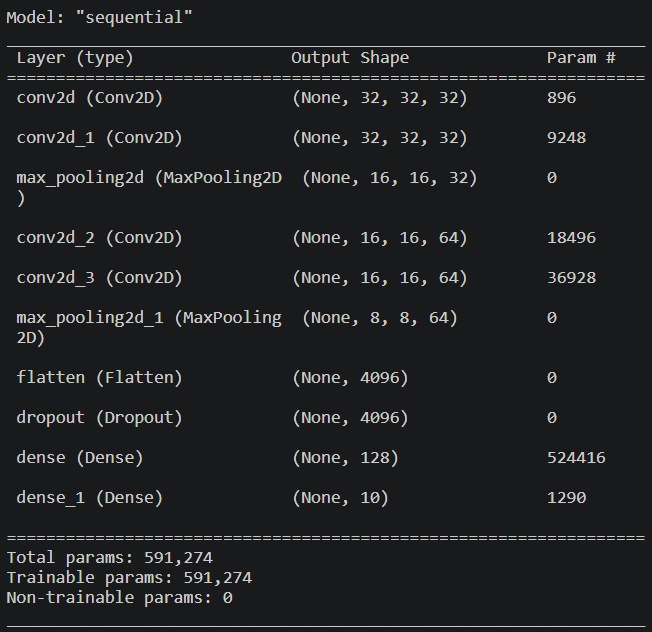
\includegraphics[width=\textwidth]{Assets/1.png}
    \caption*{Model Architecture}
  \end{minipage}
  % \centering
\end{figure}

\subsection{ReLU vs tanh vs sigmoid}

In this assignment, we compared the performance of three different activation functions using the Adam optimizer. We trained the model for 10 epochs and did not perform any hyperparameter optimization.  

Overall, our findings suggest that the choice of activation function can significantly impact the performance of the model. Further studies with hyperparameter optimization could potentially improve the performance of the model even further.

Below are the obtained results (values approximated for better comparison):

\begin{table}[H]
\centering
\begin{tabular}{||c | c | c | c ||} 
 \hline
   & ReLU & tanh & sigmoid \\ [0.5ex] 
 \hline\hline
 Training Time & 89.74 & 84.29 & 83.84 \\ 
 Classification Performance & 0.770 & 0.710 & 0.610\\[1ex] 
 \hline
\end{tabular}
\label{table:1}
\end{table}

Based on the results presented in the table, we can interpret that ReLU (Rectified Linear Unit) performs equally  than tanh (Hyperbolic Tangent) and sigmoid in terms of training time. However, when it comes to classification performance, ReLU achieves the best results, followed by tanh and sigmoid, respectively. Therefore, we can conclude that ReLU is the most suitable activation function for classification tasks.

To summarize:

\begin{itemize}
\item \textbf{Training Time:} ReLU $\approx$ tanh $\approx$ sigmoid
\item \textbf{Classification Performance:} ReLU $>$ tanh $>$ sigmoid
\end{itemize}

It is important to note that the results may vary depending on the specific dataset and model architecture used. Nonetheless, based on the findings of this experiment, \textbf{ReLU appears to be the best choice for achieving high classification performance while minimizing training time.}

\subsection{Momentum and Adaptive Learning}
After experimenting with different activation functions and optimization algorithms, we found that using ReLU as the activation function gives the best results. We compared three different optimization algorithms: SGD without momentum, SGD with momentum, and Adam. The results are summarized in the table below.

\begin{table}[H]
\centering
\begin{tabular}{||c | c | c | c ||} 
 \hline
   & SGD(w/o momentum) & SGD (with momentum) & Adaptive Learning (Adam)\\ [0.5ex] 
 \hline\hline
 Training Time & 76.64 & 77.41 & 89.74 \\ 
 Classification Performance & 0.504 & 0.758 & 0.770\\[1ex] 
 \hline
\end{tabular}
\label{table:1}
\end{table}

We found that the model with momentum outperformed the model without momentum in terms of classification performance. Furthermore, the model with momentum achieved this improvement in accuracy with only a slight increase in training time. However, the Adaptive Learning model outperformed both SGD and SGD with momentum, achieving the highest classification performance while still maintaining a reasonable training time increment.

\textbf{Based on these results, we recommend using an architecture with ReLU as the activation function and Adam (or any other Adaptive Learning model) as an optimizer for this task.}


\par\noindent\rule{\textwidth}{0.4pt}
\pagebreak
%%%%%%%%%%%%%%%%%%%%%%%%%%%%%%%%%%%%%%%%%%
%%%%%%%%%%%%%%%%%%%%%%%%%%%%%%%%%%%%%%%%%%
%%%%%%%%%%%%%%%%%%%%%%%%%%%%%%%%%%%%%%%%%%
%%%%%%%%%%%%%%%%%%%%%%%%%%%%%%%%%%%%%%%%%%
\section{CNN as a feature extractor}
\subsection{DATASET : Multi-class Weather Dataset}
The Multi-class Weather Dataset is a collection of images of various weather conditions that can be used for image classification tasks. This dataset contains a total of 1125 images of four different weather categories, namely Sunny, Cloudy, Rainy, and Snowy.

Each category contains an approximately equal number of images, i.e., around 275 images per category. The images are taken from various locations and angles, including aerial shots and ground-level images, and were captured by different cameras and photographers.
\par\noindent\rule{\textwidth}{0.4pt}
\pagebreak
%%%%%%%%%%%%%%%%%%%%%%%%%%%%%%%%%%%%%%%%%%
%%%%%%%%%%%%%%%%%%%%%%%%%%%%%%%%%%%%%%%%%%
%%%%%%%%%%%%%%%%%%%%%%%%%%%%%%%%%%%%%%%%%%
%%%%%%%%%%%%%%%%%%%%%%%%%%%%%%%%%%%%%%%%%%
\section{YOLO V2 }
YOLO V2, an improved version of YOLO, was introduced in 2017 with several new features that improved its accuracy and speed. 5 additional Features of YOLO V2:
\begin{enumerate}
\item \textbf{Anchor boxes}: YOLO V2 introduced anchor boxes, which are pre-defined bounding boxes that are used to better detect objects of different sizes and aspect ratios. Anchor boxes provide more flexibility and accuracy than the grid cells used in YOLO V1, which were fixed in size and aspect ratio.
\item \textbf{Darknet-19 architecture}: YOLO V2 uses the Darknet-19 architecture, which is a smaller and faster version of the original Darknet architecture used in YOLO V1. Darknet-19 uses fewer convolutional layers than Darknet, but still provides high accuracy and detection performance.
\item \textbf{Batch normalization}: YOLO V2 uses batch normalization, a technique that normalizes the inputs to each layer of the neural network. Batch normalization helps to reduce the effects of internal covariate shift and improves the stability and speed of the training process.
\item \textbf{Multi-scale training}: YOLO V2 uses multi-scale training, which involves training the neural network on images of different sizes. This allows YOLO V2 to better detect objects of different scales and sizes in the same image.
\item \textbf{Softmax classifier}: YOLO V2 uses a softmax classifier to predict the class probabilities of objects in each grid cell. The softmax classifier provides more accurate and reliable class predictions than the logistic regression classifier used in YOLO V1.
\end{enumerate}
\par\noindent\rule{\textwidth}{0.4pt}
\pagebreak
%%%%%%%%%%%%%%%%%%%%%%%%%%%%%%%%%%%%%%%%%%
%%%%%%%%%%%%%%%%%%%%%%%%%%%%%%%%%%%%%%%%%%
%%%%%%%%%%%%%%%%%%%%%%%%%%%%%%%%%%%%%%%%%%
%%%%%%%%%%%%%%%%%%%%%%%%%%%%%%%%%%%%%%%%%%
\section{Object tracker: SORT + DeepSORT}
\par\noindent\rule{\textwidth}{0.4pt}
\end{document} 